\section{Parametric Pipeline}

A pipeline is a collection of stages and control flow edges. Each stage can be
thought of as a function that operates over one or more inputs and returns an 
output. The datatype that flows between stages is called the Context.

A pipeline computes
by moving a generic data structure, called the Context, between 

The pipeline is composed of seven stages: Arrival, Extraction, Choice, 
Selection, Execution, Group, and Egress. Stages are connected together to
form a directed graph


\begin{figure}[h]
  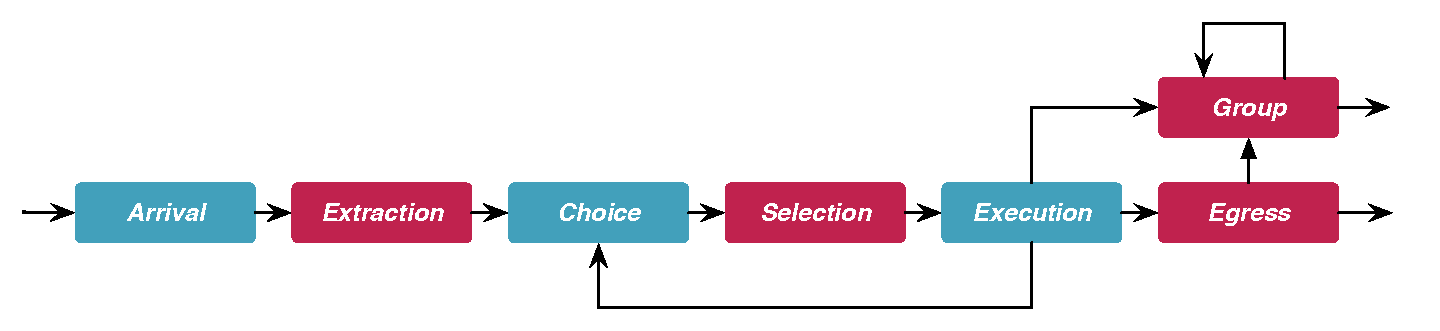
\includegraphics[width=\linewidth]{figures/pipeline.pdf}
  \label{figure:pipeline}
  \caption{FlowSim Switch Pipeline}
\end{figure}

\begin{figure}
  \lstinputlisting{code/context.steve}
  \label{listing:context}
  \caption{Context Datatype}
\end{figure}

\begin{figure}
  \lstinputlisting{code/internal.steve}
  \label{listing:internal}
  \caption{Internal Datatype}
\end{figure}
